\documentclass[leqno]{article}
\usepackage[utf8]{inputenc}
\usepackage{lscape}
\usepackage{natbib}
\usepackage{graphicx}
\usepackage{amsmath}
\usepackage{multirow}
\usepackage{multicol}
\usepackage{color, soul}
\usepackage{comment}
\usepackage{subcaption}
\usepackage{tabularx}
\usepackage{float}
\usepackage[toc,page]{appendix}
\usepackage{setspace}
\usepackage{footmisc}
\usepackage{threeparttable}
\usepackage{longtable}
\usepackage{booktabs}
\usepackage{caption}
\usepackage{abstract}
\renewcommand{\abstractname}{}    % clear the title
\renewcommand{\absnamepos}{empty} % originally center
\usepackage{float}

\usepackage[absolute,overlay]{textpos}


\usepackage{natbib}
\usepackage[authordate,backend=biber]{biblatex-chicago}
\usepackage{biblatex}
\addbibresource{bib.bib}


\usepackage{hyperref}
\hypersetup{
    colorlinks=true,
    linkcolor=blue,
    filecolor=magenta,      
    urlcolor=cyan,
    allcolors=blue
    }


\usepackage[margin=1in]{geometry}

\renewcommand{\baselinestretch}{1.5}
\renewcommand{\arraystretch}{1.5}
\renewcommand{\footnotelayout}{\setstretch{1.5}}
\title{PS11}

\title{%
  PS11 \\
  \Large A Study on the Fuel Cost Competition based on LNG Introduction Method in the Korean LNG Electricity Generation Market}

    
    
\date{April 2024}

\begin{document}

\maketitle



\section{Introduction}

In the global LNG market, the Seller's market, where suppliers have an advantage according to supply and demand conditions, and the Buyer's market, where consumers have an advantage, have been repeated. Buyer's market has a low LNG market price due to a high LNG supply (oversupply) or lack of demand, and Seller's market has a high LNG market price due to a lack of LNG supply or high demand. 

Korea's LNG generators compete for fuel cost and efficiency in the cost-based pool (CBP) electricity generation market and are mainly responsible for the peak load. Until now, most LNG generators in Korea have been supplied with LNG from the Korea Gas Corporation(KOGAS). Meanwhile, since the start of the Buyer's market, which has a low global LNG market price since 2015, the number of generators that directly purchase and procure LNG from overseas without receiving LNG for electricity generation from KOGAS has been increasing. This is in accordance with the purpose of securing a cost advantage in the LNG electricity generation competition in the Korean electricity market by directly introducing inexpensive LNG in the global LNG market from 2015.

KOGAS, which supplies about 82\% of LNG introduced to Korea, values stable procurement of supplies. Therefore, it is characterized by a high proportion of long-term contracts based on oil price linkage that can stably procure the quantity. On the other hand, it is known that private direct-import electricity generation companies are very sensitive to the introduction of LNG prices and have a low proportion of long-term contracts compared to KOGAS because they pursue profits. Consequently, private direct-import electricity generation companies have a high proportion of the LNG spot market. In particular, it has been known that in the buyer's market, private direct-import electricity generation companies showed a cost advantage over KOGAS because the spot market price is low. However, as the global LNG market was converted to the seller's market due to the energy crisis that occurred before and after the outbreak of the Russian-Ukrain War, the LNG spot market price rose to the highest after the LNG transaction, and the high price continued. During this period, it can be estimated that  KOGAS electricity generation with a small proportion of the spot volume will have a cost advantage over LNG direct imported generators.

The purpose of this study is to analyze empirically whether private electricity generators directly importing LNG are advantageous in terms of cost during the Buyer's market period in the Korean electricity market and whether KOGAS generators are advantageous in terms of cost in the Seller's market. To this end, Chapter 2 examines literature studies related to the natural gas pricing mechanism and gas introduction competition in the electricity market. And, we will examine the current status of Korea's LNG introduction competition and electricity generation competition market. In the analysis part of Chapter 3, we will distinguish between Buyer's market and Seller's market by analyzing the current Asian LNG price (JKM, Japan Korea Market) from January 2015 to May 2023, when LNG direct introduction generators appeared in earnest, using Bai Parron's test to determine whether there is a structural change in market price. In chapter 4, We provide empirical results. The last chapter will discuss this study's main results, implications, and limitations.

\section{Institutional Background}

\subsection{Literature Review}



\subsection{Current Situation of Korea's LNG introduction competition and Electricity Generation Competition Market}


Figure1 \footnote{Data Source: S\&P 2024, Global Commodity Insights, Japan Ministry of Finance, China Customs}

\begin{figure}[htbp] 
    \centering
            \caption{Global Gas and LNG Prices(\$/MMBtu)}
        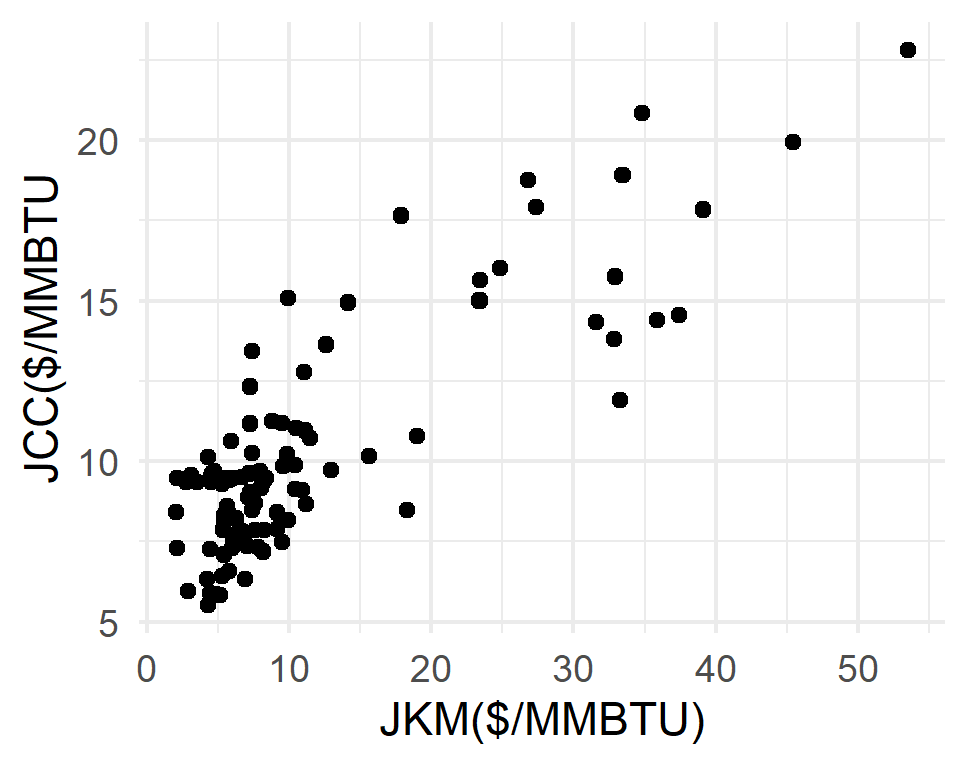
\includegraphics[width=0.8\linewidth]{Figure1.png}
        \label{fig:88mono}
\end{figure}




\section{Data and Empirical Strategy}

\subsection{Data Description}
The purpose of this study is to empirically analyze whether generators directly importing LNG are advantageous in terms of cost during the Buyer's market period within the Korean electricity market, and whether KOGAS generators(importing jointly) are advantageous in terms of cost in the Seller's market. To this end, 8,420 panel data per month for 91 LNG generators were constructed from January 2015 to May 2023. The data is from the Korea Electric Power Corporation(KEPCO), and consists of the generator name, year, month, monthly fuel price for generators in generating electricity, LNG generator type, fuel introduction method (KOGAS; average price, Private; direct import, Combination; both), JKM price, JCC price, HH price, terminal ownership, and generator capacity. There are 800 data for the direct import method, 7,428 data for the average price for KOGAS, and 192 data for combination. Table below provides basic statistics on 8420 data used in this analysis. The average fuel price for the entire sample period was 64 won, JKM was 12 dollars, and JCC was 10 dollars.





\begin{table}[htbp]\centering
\def\sym#1{\ifmmode^{#1}\else\(^{#1}\)\fi}
\caption{Summary Stats}
\begin{tabular}{l*{1}{ccccc}}
\toprule
\addlinespace
\textsc{Statistic}            &        \multicolumn{1}{c}{\textsc{Mean}}&         \multicolumn{1}{c}{\textsc{St. Dev.}}&        \multicolumn{1}{c}{\textsc{Min}}&         \multicolumn{1}{c}{\textsc{Max}}&           \multicolumn{1}{c}{\textsc{N}}\\
\hline \hline
\addlinespace
Fuel Price       &    64.03&    31.53&      16.89&       308.9&        8420\\
JKM         &    12.06&    10.79&       2.06&      53.51&        8420\\
JCC         &    10.48 &    3.65&        5.52&        22.8&        8420\\
HH          &    3.28&    1.51 &         1.7&        8.81&        8420\\
Capacity    &    421.19&    220.39&          21&         874&        8420\\
\bottomrule
\end{tabular}
\end{table}


The fuel price can be composed of the raw material cost and the supply cost. The raw material cost is the price of LNG introduction. The supply cost is calculated based on the LNG terminal rate and the piping cost. Of the total fuel price, the proportion of raw material accounts for 90\% and the proportion of supply cost accounts for about 10\%, indicating that the influence of raw material is absolute (Hong, 2021).

\begin{figure}[htbp] 
    \centering
            \caption{Fuel Price and JKM(\$/MMBtu) by LNG Import Type}
        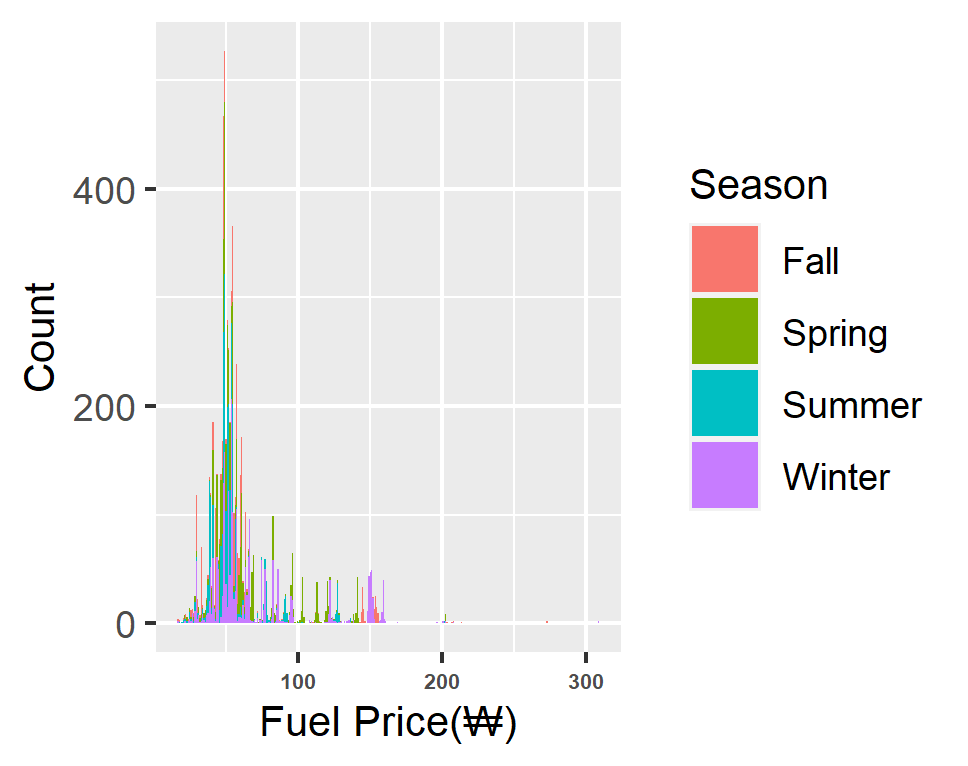
\includegraphics[width=0.5\linewidth]{Figure3.png}
        \label{fig:88mono}
\end{figure}

\begin{figure}[htbp] 
    \centering
            \caption{Fuel Price and JCC(\$/bbl) by LNG Import Type}
        \includegraphics[width=0.5\linewidth]{Figure4.png}
        \label{fig:88mono}
\end{figure}

\begin{figure}[htbp] 
    \centering
            \caption{Fuel Price Histogram by Season}
        \includegraphics[width=0.5\linewidth]{Figure5.png}
        \label{fig:88mono}
\end{figure}


\subsection{Dividing Buyer's-Seller's Market using Bai-Perron Method}


In this study, first, the Bai-Perron (1998, 2003) test was used to analyze whether there was a structural change in the LNG market price using monthly data of the Asian LNG spot price, Japan-Korea Marker (JKM), from January 2015 to May 2023. Figure below visualizes the price trend of JKM Price. Starting in mid-2021, it can be seen that JKM prices rise sharply.


\begin{figure}[htbp] 
    \centering
            \caption{JKM Price and Structural Break(\$/MMBtu}
        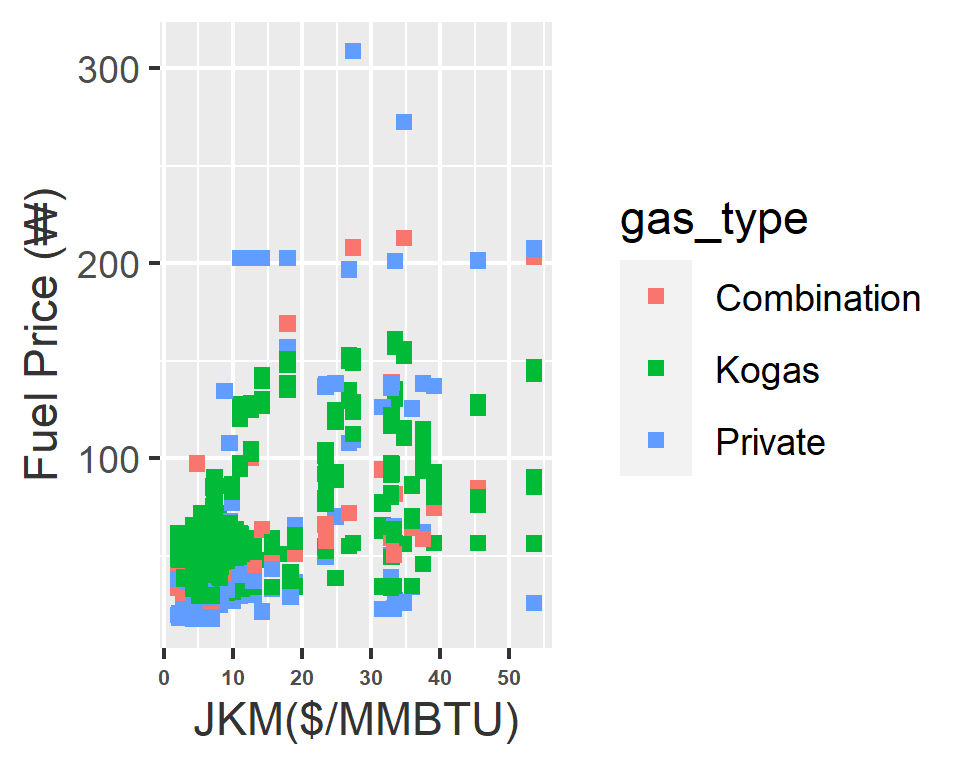
\includegraphics[width=0.6\linewidth]{Figure2.png}
        \label{fig:88mono}
\end{figure}






\subsection{Empirical Approach}

In this study, the regression analysis model is set as the model to analyze which method is more cost-effective for the fuel price between the direct introduction private generator and the KOGAS generator with average price.


\cite{bai1998estimating}
\cite{bai2003computation}
\cite{bai2003critical}


\section{Baseline Findings}

\subsection{Basic Result}
The table below shows the results of the basic regression analysis. Regression 1 table is the result of the model that considers only year-seasonal and generator-type fixed effects without including control variables. As a result of the analysis, it was found that the fuel price of the directly imported private generator was significantly more cost-effective than that of the KOGAS(average price) generator. The mixed generator(combination) fuel price is significantly reduced, but the magnitude is relatively smaller than directly imported private generators.


\begin{table}[htbp]\centering
\def\sym#1{\ifmmode^{#1}\else\(^{#1}\)\fi}
\caption{Regression Result 1\label{tab1}}
\begin{tabular}{l*{1}{c}}
\toprule
 & \multicolumn{1}{c}{\textsc{Dependent variable}} \\ 
                     &\multicolumn{1}{c}{\textsc{:Fuel Price}}\\
                     \addlinespace
\hline \hline
\addlinespace
\textit{Combination} \small{(Kogas+direct Import)}          &      -4.524\sym{***}\\
                    &      (0.89)         \\
\addlinespace
\textit{Direct Import}       &     -10.861\sym{***}\\
                    &      (0.45)         \\
\midrule
Year-Season FE        &    Yes \\  
Generator Type FE        &    Yes \\  
Observations                   &    8420         \\
$R^2$                  &       0.853         \\
\hline \hline
\multicolumn{2}{l}{\footnotesize Standard errors in parentheses}\\
\multicolumn{2}{l}{\footnotesize \sym{*} \(p<0.1\), \sym{**} \(p<0.05\), \sym{***} \(p<0.01\)}\\
\end{tabular}
\end{table}







\newpage
\subsection{Comparison between Buyer's Market and Seller's Market}


\begin{table}[h]\centering
\def\sym#1{\ifmmode^{#1}\else\(^{#1}\)\fi}
\caption{Regression Result 2\label{tab1}}
\begin{tabular}{l*{4}{c}}
\toprule
 & \multicolumn{4}{c}{\textsc{Dependent variable}} \\ 
                     &\multicolumn{4}{c}{\textsc{:Fuel Price}}\\
                                          \cline{2-5}  \\
                    &\multicolumn{1}{c}{(1)}&\multicolumn{1}{c}{(2)}&\multicolumn{1}{c}{(3)}&\multicolumn{1}{c}{(4)}\\
\hline \hline
\addlinespace
\textit{Combination} \small{(Kogas+Direct Import)}          &      -4.526\sym{***}&      -5.034\sym{***}&      -4.505\sym{***}&      -4.510\sym{***}\\
                    &      (0.86)         &      (0.88)         &      (0.86)         &      (0.77)         \\
\addlinespace
\textit{Direct Import}        &     -10.860\sym{***}&     -10.726\sym{***}&     -10.825\sym{***}&     -10.834\sym{***}\\
                    &      (0.44)         &      (0.47)         &      (0.45)         &      (0.41)         \\
\addlinespace
JKM                 &      -0.262\sym{***}&      -0.262\sym{***}&      -0.262\sym{***}&       \textit{omitted}         \\
                    &      (0.04)         &      (0.04)         &      (0.04)         &                  \\
\addlinespace
JCC                 &       4.935\sym{***}&       4.935\sym{***}&       4.935\sym{***}&       \textit{omitted}         \\
                    &      (0.20)         &      (0.20)         &      (0.20)         &                  \\
\addlinespace
Capacity            &                     &                     &      -0.000         &      -0.000         \\
                    &                     &                     &      (0.00)         &      (0.00)         \\
\midrule
Year-Season FE         &    Yes &    Yes&    Yes&    No\\  
Generator Type FE        &    Yes &    Yes&    Yes&    Yes\\  
Capacity Interval FE    &   No &    Yes&    No&    No\\  
Year-Month FE        &    No &    No&    No&    Yes\\  
Observations                   &    8420         &   8420        &    8420         &    8420        \\
$R^2$                  &        0.864         &      0.865          &        0.864          &        0.892         \\
\hline \hline
\multicolumn{5}{l}{\footnotesize Standard errors in parentheses}\\
\multicolumn{5}{l}{\footnotesize \sym{*} \(p<0.1\), \sym{**} \(p<0.05\), \sym{***} \(p<0.01\)}\\
\end{tabular}
\end{table}


\begin{table}[h]\centering
\def\sym#1{\ifmmode^{#1}\else\(^{#1}\)\fi}
\caption{Buyer's Market and Seller's Market\label{tab1}}
\begin{tabular}{l*{3}{c}}
\toprule
 & \multicolumn{3}{c}{\textsc{Dependent variable}} \\ 
                     &\multicolumn{3}{c}{\textsc{:Fuel Price}}\\
                                          \cline{2-4}  \\
                  &\multicolumn{1}{c}{\textsc{Overall}}&\multicolumn{1}{c}{\textsc{Buyer's}}&\multicolumn{1}{c}{\textsc{Seller's}}\\           
                 &\multicolumn{1}{c}{\textsc{Sample Period}}&\multicolumn{1}{c}{\textsc{Market}}&\multicolumn{1}{c}{\textsc{Market}}\\     
                    &\multicolumn{1}{c}{(1)}&\multicolumn{1}{c}{(2)}&\multicolumn{1}{c}{(3)}\\

\hline \hline
\addlinespace
\textit{Combination} \small{(Kogas+Direct Import)}          &      -4.505\sym{***}&      -2.657\sym{***}&      -8.417\sym{***}\\
                    &      (0.86)         &      (0.47)         &      (2.52)         \\
\addlinespace
\textit{Direct Import}        &     -10.825\sym{***}&     -10.093\sym{***}&     -12.694\sym{***}\\
                    &      (0.45)         &      (0.23)         &      (1.52)         \\
\addlinespace
JKM                 &      -0.262\sym{***}&      -0.084         &      -0.426\sym{***}\\
                    &      (0.04)         &      (0.05)         &      (0.09)         \\
\addlinespace
JCC                 &       4.935\sym{***}&       3.330\sym{***}&       6.140\sym{***}\\
                    &      (0.20)         &      (0.14)         &      (0.48)         \\
\addlinespace
Capacity            &      -0.000         &      -0.001\sym{**} &       0.002         \\
                    &      (0.00)         &      (0.00)         &      (0.00)         \\
\midrule
Observations                   &    8420         &    6244         &    2176         \\
$R^2$                 &       0.864         &       0.760         &       0.718         \\
\hline \hline
\multicolumn{4}{l}{\footnotesize Standard errors in parentheses}\\
\multicolumn{4}{l}{\footnotesize \sym{*} \(p<0.1\), \sym{**} \(p<0.05\), \sym{***} \(p<0.01\)}\\
\end{tabular}
\end{table}




\newpage
\subsection{Price Cap Regulation Impact}


\subsection{Terminal Ownership Effect}

\newpage
\subsection{Robstness Checks}


\newpage
\section{Discussion and Conclusion}
In this study, we expected that private generators directly importing LNG with a low proportion of long-term contracts and a high proportion of spot goods would be advantageous in the buyer's advantage market, and that generators importing from KOGAS with a high proportion of long-term contracts and a low proportion of spot goods would have a cost advantage in the seller's advantage market. This is because the spot gas market price is low in the seller's advantage market, and the spot gas market price is high in the buyer's advantage market. However, contrary to our expectations, private generators directly importing LNG showed a cost advantage over KOGAS generators in both the buyer's market and the seller's market. It was even found that the cost competitiveness was higher in the buyer's advantage market than in the seller's advantage market. This can be interpreted as several reasons.

Firstly, 

Secondly, 


\newpage
\printbibliography

\end{document}
